\documentclass{beamer}
\usepackage{lsfolien}
\usepackage[english]{babel}

\myfootline{Sustainability, Environment, Management -- Summer Term
  2022}{Hans-Gert Gr\"abe}

\title{Business Model Patterns and Sustainability\vskip1em}

\subtitle{Research Seminar in the Module 10-202-2312\\ for Master Computer
  Science}

\author{Prof. Dr. Hans-Gert Gräbe\\
\url{http://www.informatik.uni-leipzig.de/~graebe}}

\date{June 2022}
\begin{document}

{\setbeamertemplate{footline}{}
\begin{frame}
  \titlepage
\end{frame}}

\begin{frame}{Institutionalisation and Technology}

  \begin{block}{What is Technology?}
    Technology is an interrelation of
    \begin{itemize}
    \item globally available \emph{procedural knowledge}, 
    \item \emph{institutionalised procedures} ("state of the art") and
    \item private \emph{procedural skills}.
    \end{itemize}
  \end{block}
\end{frame}

\begin{frame}{The TRIZ Way of Thinking}
\small
  \begin{center}
  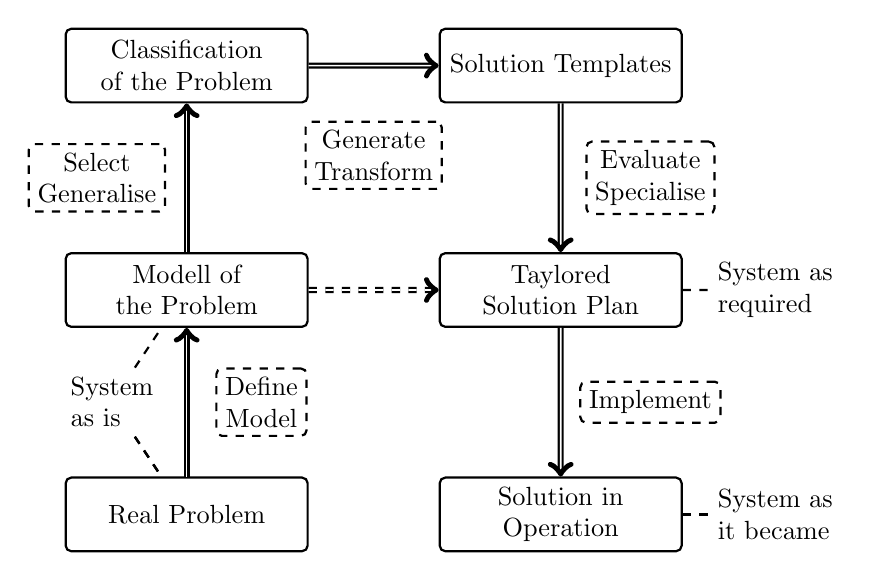
\begin{tikzpicture}[scale=.95,transform shape,
      textbox/.style={draw, text width=3cm, minimum height=2.8em,
        align=center},
      ovalbox/.style={draw, dashed, align=center},
      %>={Triangle[length=0pt 6,width=0pt 5]},
      rounded corners=2pt,line width=.8pt]

    \node[text width=1.1cm] at (-1,1.5) (A0) {System\\ as is};
    \node[textbox] at (0,0) (A1) {Real Problem};
    \node[ovalbox] at (1,1.5) {Define\\ Model}; 
    \node[textbox] at (0,3) (A2) {Modell of the Problem};
    \node[ovalbox] at (-1.2,4.5) {Select\\ Generalise}; 
    \node[textbox] at (0,6) (A3) {Classification of the Problem};
    \node[ovalbox] at (2.5,4.8) {Generate\\ Transform}; 
    \node[textbox] at (5,6) (B3) {Solution Templates};
    \node[ovalbox] at (6.2,4.5) {Evaluate\\ Specialise}; 
    \node[textbox] at (5,3) (B2) {Taylored\\ Solution Plan};
    \node[ovalbox] at (6.2,1.5) {Implement}; 
    \node[textbox] at (5,0) (B1) {Solution in Operation};
    \node[text width=1.8cm] at (8,3) (C2) {System as\\ required};
    \node[text width=1.8cm] at (8,0) (C1) {System as\\ it became};

    \draw[-,dashed] (A0) -- (A1);
    \draw[-,dashed] (A0) -- (A2);
    \draw[-,dashed] (B1) -- (C1);
    \draw[-,dashed] (B2) -- (C2);
    \draw[-,dashed] (A0) -- (A1);
    \draw[-,dashed] (A0) -- (A1);
    
    \draw[double,->] (A1) -- (A2) ;
    \draw[double,->] (A2) -- (A3) ;
    \draw[double,->] (A3) -- (B3) ;
    \draw[double,->,dashed] (A2) -- (B2) ;
    \draw[double,->] (B3) -- (B2) ;
    \draw[double,->] (B2) -- (B1) ;
\end{tikzpicture}
\end{center}
\end{frame}

\begin{frame}{Patterns and Contexts}

  These forms of institutionalisation are embedded as initially domain-specific
patterns in a \emph{domain-specific} methodology, for example as industry
sector-specific standards and thus are \emph{contextualised}.

These patterns can be further generalised to cross-domain standards such as
the APQC PCF as a Cross-Industry Process Classification Framework.

However, this is also \emph{not universally valid}, but contextualised itself,
as it still refers to organisations of a specific-general design.

\end{frame}

\begin{frame}{TRIZ and Patterns}

TRIZ is similarly structured. It comes with a toolbox of problem-solving
patterns (Select in [Mann])

\begin{itemize}
\item[] Inventive principles, Separation Principles, ...
\end{itemize}
but assumes a specific type of modelling (Define in [Mann]) with
\begin{itemize}
\item[] Systemic delimitation, Ideality, Operative Zone, ...
\end{itemize}
Only on the basis of this (Define) the (Select) is possible. 
\end{frame}

\begin{frame}{Development of Business Process Modelling}
  \begin{itemize}
  \item Modelling of work processes (patterns, roles, qualification, ...) 
  \item Business Process Modelling
  \item Business Models (P-TRIZ level according to Howard Smith)
  \end{itemize}

  Business Process Models and Business Models\vskip1em

  \begin{block}{What is a Pattern?}
    A pattern is a combination of a problem and a corresponding solution that
    is described in a systematic and generic way, so that it can be used over
    and over again in different situations.
  \end{block}
  
\end{frame}

\begin{frame}{Sustainability Emerging as Business Goal}

\begin{center}
  \includegraphics[width=.8\textwidth]{images/SDG.png}
\end{center}\vspace*{-4em}

\emph{Vision 2050. It's time to transform.} Published by the World Business
Councel for Sustainable Development.

\end{frame}

\begin{frame}{Sustainability and Business Models}
\begin{center}
  \begin{minipage}{.4\textwidth}\centering
    \includegraphics[width=\textwidth]{images/Triple-Bottom-Line.png}\\
    Triple Bottom Line
  \end{minipage}
  \begin{minipage}{.55\textwidth}
    A business model for sustainability “helps describing, analyzing,
    managing, and communicating
  \begin{itemize}
  \item[(i)] a company’s sustainable value proposition to its customers, and
    all other stakeholders,
  \item[(ii)] how it creates and delivers this value,
  \item[(iii)] and how it captures economic value while maintaining or
    regenerating natural, social, and economic capital beyond its
    organizational boundaries”.
  \end{itemize}
  [Schaltegger et al. 2016]
  \end{minipage}
\end{center}
\end{frame}

\begin{frame}{Sustainability and Business Models}

  [Lüdeke-Freund et al. 2018]
  
The authors extraced 45 patterns from the literature on Sustainable Business
Models and grouped them into 11 pattern groups.

Example: Pattern group \emph{Pricing \& Revenue Patterns}
\begin{itemize}
\item Differential Pricing
\item Freemium
\item Innovative Product Financing
\item Subscription Model
\end{itemize}
\end{frame}

\begin{frame}{Sustainability and Business Models}
Description of \emph{Differential Pricing}
\begin{itemize}
\item \emph{Context:} Base of the Pyramid and low-income groups in both
  developed and developing countries are often excluded from consumption due
  to price barriers.
\item \emph{Problem:} Customers might need the same product but have different
  payment thresholds. Hence, some customers are either unwilling or unable to
  pay as much as others for the same product.
\item \emph{Solution:} Charging groups with higher payment thresholds higher
  prices to subsidize those groups who cannot afford to pay as much.
\item \emph{Example:} [Novo Nordisk] sells insulin in developing countries at
  prices that are up to 20\% below the mean prices charged in developed
  countries.
\end{itemize}
\end{frame}

\begin{frame}{Sustainability and Business Models}
  General purpose idea generation tools (including TRIZ -- HGG) do not usually
  show any specific preference to sustainable aspects, since their overall
  purpose is product success and the identification of unexplored market
  opportunities.  Therefore, the attention to sustainability is random, not
  taken for granted and presumably dependent on designers’ sensibilities
  towards environmental and human problems. [Russo, Spreafico 2020]
\end{frame}

\begin{frame}{Lifecycle Orientation and Eco Design Principles}

  [Russo, Spreafico 2020]

General orientation of the \emph{Eco Design Principles} (EDP) approach:
\begin{quote}
  During design phase, each designer is supposed to follow a list of
  guidelines and accordingly modify the existing product to make it more
  environmentally friendly. The crucial point is to exploit problem solving
  strategies as a framework for eco-guidelines that guide the user to make
  product development, taking into account first of all sustainability
  objectives.
\end{quote}

\textbf{16 generic strategies} are derived, to which the identified 59 Eco
Guidelines are assigned.

\end{frame}

\begin{frame}{Lifecycle Orientation and Eco Design Principles}
Each of these generic strategies is embedded in the TRIZ methodology and their
solving power is outlined \emph{without, however, assigning them to a
  problem}.
  
Example: Strategy 2 \emph{Trimming}:
\begin{quote}
  Trimming is a good technique for making greener products. It consists of
  making a product constituted by fewer parts, with positive consequences on
  many aspects of the product life cycle, from the management of warehouse
  orders, storage, transport, as well as on reducing the mass. In order to
  achieve the maximum environmental benefits, it is preferable to start by
  eliminating those pieces having the highest impact on the environment. When
  a component is deleted from the system, it is better to try to exploit the
  resources already available in the super-system to replace its useful
  function.
\end{quote}

\end{frame}

\begin{frame}{Lifecycle Orientation and Eco Design Principles}
  
The description of each principle is limited to a detailed \emph{Generic
  Suggestion}, more structured \emph{specific suggestions} and examples.

Similar to [Gassmann et al. 2014], the individual EDPs are also assigned
values from a morphological table with the attributes \emph{when, action,
  what, how}.
\begin{itemize}
\item \emph{When:} Premanufacturing, Manufacturing, Use, End of Life
\item \emph{Action:} Eliminate, Reduce Mass, Reduce Volume, Reduce Quantity,
  Reduce Distance, Improve Durability, Select Other.
\item \emph{What:} Raw materials, External logistics, Internal logistics,
  Packaging, Machineries, Auxiliary materials, Components, Emissions, Energy.
\item \emph{How:} Generic suggestion, Resources list, Example.
\end{itemize}

\end{frame}

\begin{frame}{Lifecycle Orientation and Eco Design Principles}

The general pattern of a guideline is formulated as 
\begin{quote}
  (WHEN) you want to intervene, (ACT) on components (WHAT), by doing
  something (HOW) and using one resource (from the Resource list) to find
  alternatives and assess environmental impacts.  
\end{quote}

In the paper the following sample of a guideline is given: 
\begin{quote}\small
  During supply task (WHEN -- Premanufacturing),\\ reduce the mass (ACTION --
  Reduce mass)\\ of the raw material (WHAT -- Raw material)\\ by recycling
  waste material in your facility to make it new raw material for the product
  (HOW -- Generic Suggestion). \\
  See list of structural resources (HOW -- Resources list)\\
  In order to reduce the mass of the casting metal, the casting channels can
  be re-used for successive melting (HOW -- Example) 
\end{quote}

\end{frame}

\begin{frame}{Eco Design Principles -- A Survey}

The authors of [Maccioni et al. 2019] conduct a literature survey on this topic.
At the beginning, the difficulties to be overcome are worked out.

Under the heading "Selection of potentially environment-friendly products"
four sources with altogether 310 products are analysed.  Based on this
analysis 66 EDPs are distinguished, giving a short description and assigning
them to the examples.

\end{frame}

\begin{frame}{Eco Design Principles -- A Survey}

Example:
\begin{itemize}
\item \emph{Product:} FRIA refrigerator, Ursula Tischner: fridge built into
  the external wall to use the winter cold.
\item \emph{Assigned EDPs:}
  \begin{itemize}
  \item P16 Minimize energy consumption gin{itemize}
  \item P18 Select non-toxic and harmless energy resources 
  \item P46 Reduce auxiliary components gin{itemize}
  \item P48 Reduce environmental problems during the product use
  \item P52 Reduce the consumption of energy required
  \end{itemize}
\item \emph{Explanation:} ‘It was calculated that in typical German house it
  could work for about 3–5 months a year without consuming any energy (P16,
  P46 and P52).’ [\ldots]
\end{itemize}

\end{frame}

\begin{frame}{Summary}\small

The SBM approach seems to be rather counterproductive, as it tries to
translate changed consumer behaviour and thus the politicisation of the
environmental problem into business models without making visible if this
leads to changes in the productive base.  In many cases it looks like seekng
new \emph{value propositions} to a prolongate an old mode of production.  

The EDP approach addresses the problem from the material side by taking
"planet" and "people" into account at an early stage of product development.
It is emphasised that TRIZ is particularly suitable as a methodology here, as
it supports both a systemic focus and provides powerful tools for analysing
and resolving contradictions.

Nevertheless the application of EDPs might lead to changes in the product
perception, boosting or undermining success chances. In the early design
phases, the product as a complex whole is not developed enough to assess that
appropriately.

\end{frame}

\end{document}
